\chapter{Numerical experiments}
\label{cha:numer-experiments}

??ds do I use h for element size elsewhere?

??ds I've never explained how to solve eBDF3 system: pin magnetostatics, mass matrix inversion, use ll equation, with nodal quadrature we have a lumped mass matrix, no inversion needed!

In this section we apply the complete FEM/BEM scheme with adaptive IMR and nodal integration, as developed in \crefs{sec:galerk-meth-llg, sec:hybr-finit-elem, sec:adaptive-imr}, to ``real-world'' micromagnetics problems.

The ??ds-th problem solved is a case where an exact solution exists.

The ??ds-th problem we tackle is the \mumag standard problem 4 \cite{mumag-website}, which is widely used to test dynamic micromagnetic codes.



\section{Wave solution}
\label{sec:numer-exper}


??ds sweep dt?

\subsection{Problem definition}

We solve the LLG without magnetostatics on a two dimensional square domain $\magd = [0,1] \times [0,1]$ with periodic boundary conditions.
In time we simulate the solution in $[0, 2]$.

In the following experiments we use the wave exact solution in 2D (see \cref{sec:wave-like-solution}) for simplicity and because an exact solution is known.
The solution parameters used are $\kvec = 2\pi$ so that the solution is periodic on domains of unit size, $c = 0.1\pi$ which gives reasonable amplitude oscillations and $\dampc = 0.01$ due to physical relevance).
For energy conservation experiments $\dampc = 0$ is used.


This problem allows us to examine the convergence and conservation properties of IMR with the FEM and nodal quadrature.
In particular the existence of an exact solution for the LLG with exchange allows us to measure the convergence rate.
Unfortunately we do not know of any non-trivial (\ie with $\mv$ varying in both space and time) exact solution for the LLG with exchange and magnetostatics.


\subsection{Implementation}

We use the finite element method as discussed in \cref{sec:galerk-meth-llg} to spatially discretise the LLG equation with exchange coupling (no other effective fields are included).
We use a mesh of square elements, % and a mesh of triangular elements made by splitting each square element in two with a diagonal line from $\sv = [0, 1]$ to $\sv = [1, 0]$.
unless otherwise specified we use a mesh with $5 \times 2^4$ elements along each edge.

Both the nodal quadrature discussed in \cref{sec:local-nodal-integr} and standard Gaussian quadrature are used in order to compare the two.

For time integration the IMR, TR and BDF2 methods are used, adaptive step sizes with a tolerance of $\toltt = 10^{-5}$ are used except for the convergence experiment which requires fixed step sizes.

Linearisation is handled using the Newton-Raphson method, the newton tolerance is set to $10^{-12}$ unless otherwise specified.
The linear systems are solved using GMRES with an ILU-1 preconditioner.\footnote{\hypre's Euclid preconditioner \cite{hypre} with no drop tolerance and factorisation level 1.}


\subsection{General results}


An example snapshot of the solution is shown in \cref{fig:2d-wave-snapshot}.
As time proceeds the wave moves in the $[1,1]$ direction and is simultaneous damped out to the $\mv = [0,0,1]$ state.
Time plots of the exact solution along with more details are given in \cref{sec:wave-like-solution}.

\begin{figure}
  \centering
  
\includegraphics[width=0.8\textwidth]{images/placeholder}
  \caption{Snapshot of the solution}
  \label{fig:2d-wave-snapshot}
\end{figure}


??ds example time trace?

??ds These choices of mesh and time step resolve the solution well, as can be seen in the convergence experiments above.

The time step behaviour for this problem is simple: all of the integrators rapidly increase the time step to a reasonable value then keep it roughly constant (increasing slightly in the damped case).
This is as expected, in particular note that there is no oscillation of the step size with the precessional motion unlike in \cref{sec:aimr-llgode-numerical-results}.


??ds TR catastrophic failure?


\subsection{Accuracy of nodal quadrature}

??ds do this?



\subsection{Convergence}

Since we have an exact solution for this example we can calculate the total error and plot the convergence as $\dtn \goesto 0$ and $h \goesto 0$.
Following the example of Jeong \etal \cite{Jeong2014} we link the spatial discretisation length to the time step by $\dtn = 0.32h$. (Note that in contrast to explicit time integration methods this is \emph{not} required for stability it is merely more convenient to experiment with a single parameter.)
We set $h = 1/5(2^n)$ with $n=1,2,3,4,5,6,7,8 ??ds$.

The error norm used is $\errmpde = \norm{m(\xv_j, t_n) - \mv_j,n}$. ??ds this is no good...

We plot two figures: the error after a single step and the error after some time.

??ds


\subsection{Conservation properties}
\label{sec:2d-wave-results-cons-prop}

% The maximum time was $t_{max} = 5$ ($\approx 20$ wave periods), the damping is small enough that the oscillations continue well past this time. % trace in folder ??ds check it
\Cref{fig:mean-ml-error-2d} shows the behaviour of the maximum (over all nodes) error in magnetisation length.
When using (adaptive) IMR with nodal quadrature the magnetisation length error remains extremely small ($\order{10^{-14}}$).
When using IMR with Gaussian quadrature or BDF2 the error rapidly grows to around $\order{10^{-4}}$ and remains there.
It is interesting to note that nodal integration has a slight beneficial effect on the magnetisation length error of BDF2.

\begin{figure}
  \centering
  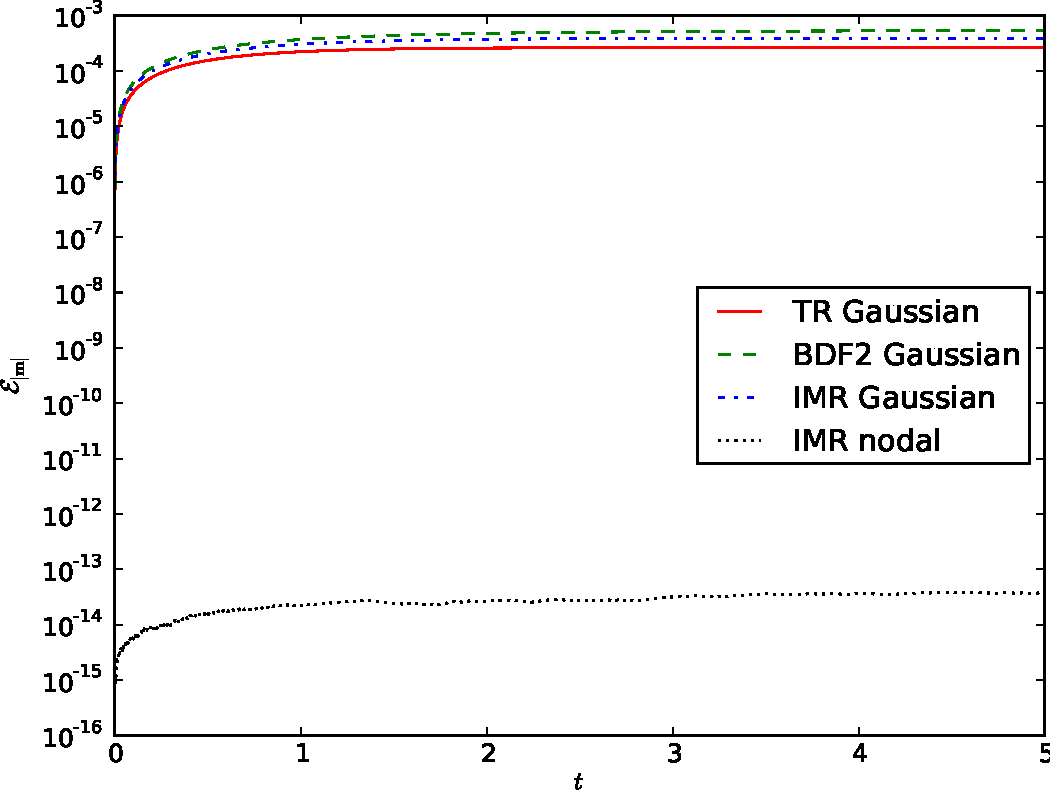
\includegraphics[width=0.8\textwidth]{plots/2d_wave_solution_m_length/mlengtherrormaxesvstimes}
  \caption{Evolution of the maximum error of nodal magnetisation lengths in the 2D wave example with various time integrators and quadratures.}
  \label{fig:mean-ml-error-2d}
\end{figure}

 % ??ds rerun this?
% To check that the conservation is independent of problem parameters we ran a parameter sweep using: square and triangle elements; 36, 441 and 6561 nodes; time steps of $0.1$, $0.01$ and $0.001$; and damping parameters of $1$, $0.1$, $0.001$ and $0$.
% The maximum length error over all parameter sets, all time steps and all nodes when using nodal quadrature was 2.364775e-12, when using Gaussian quadrature it was 0.013746647.
% This clearly demonstrates the necessity and effectiveness of the nodal quadrature scheme for retaining the conservation properties of the implicit midpoint rule.
% % using the same data as for the figures above, look in their folders for parameter sets data parsing command: parse.py -d /mnt/moredata/optoomph/user_drivers/micromagnetics/experiments/parameter_sweeps/parameter_file_0/ -l=-dt -l=-damping --split=-integration --print-data max-max-ml --print-data ml -l=initial_nnode


We also examine the energy conservation properties of the various time integration schemes for the wave solution with $\dampc = 0$.
The energy is calculated using \cref{eq:nd-e-ex}.
The integrals can be evaluated exactly using any quadrature because $\grad \mv$ is a constant inside each element.

The results are shown in \cref{fig:energy-error-2d}.
??ds analysis

\begin{figure}
  \centering
  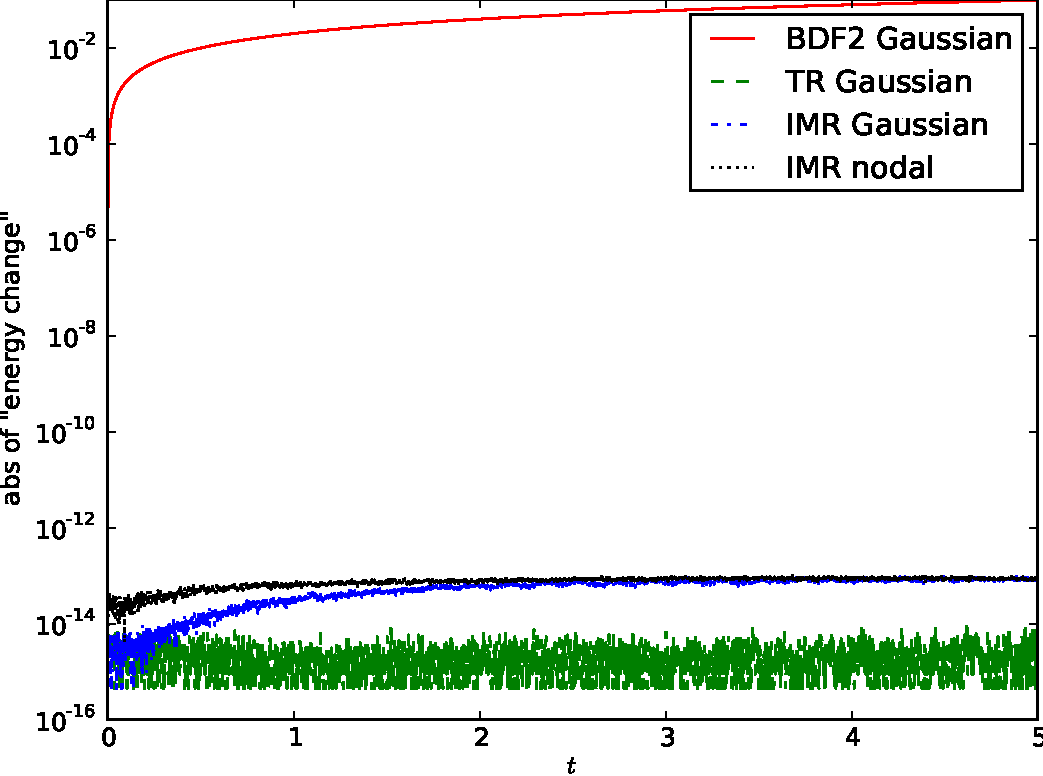
\includegraphics[width=0.8\textwidth]{plots/2d_wave_solution_energy/absofenergychangevstimes}
  \caption{Evolution of the error in energy in the undamped 2D wave example with various time integration methods, quadrature schemes and with/without re-normalisation.}
  \label{fig:energy-error-2d}
\end{figure}



\subsection{Effect of Newton tolerance}
\label{sec:effect-newt-toler-m-conservation}

Since the non-linear residual \cref{eq:weak-llg} used in the derivation of the conservation properties for energy and $\abs{\mv}$ is only true up to the accuracy of the linearisation method we would expect to see some effect when modifying this accuracy.
In our model the Newton-Raphson method is used for linearisation (see \cref{sec:newt-raph}) so the relevant measure of accuracy is the Newton tolerance, $\ntol$.

The obvious experiment to carry out would be to vary the Newton tolerance and examine how the error in $\abs{\mv}$ is affected.
However Newton's method converges extremely quickly meaning that the final residual is often orders of magnitude smaller than the tolerance, this would hide any corrolation between the tolerance and the error.
Instead we plot the error against the actual converged residual norm (specifically: the mean over time steps of $\norm{\rv}_\infty$ after the Newton method has converged).
In order to generate a variety of converged residual norms we run the experiment with a wide range of parameters: $\ntol = ??ds$, $\dtn = ??ds$, $\dampc = ??ds$ and $N_h = ??ds$.
The results are shown in \cref{fig:mean-ml-error-2d-nodal-newton-tests}, there is a clear correlation between small residuals and small $\abs{\mv}$ error.
??ds any correlation with other parameters?

A similar result is seen in \cref{} for the energy conservation property when $\dampc = 0$.

\begin{figure}
  \centering
  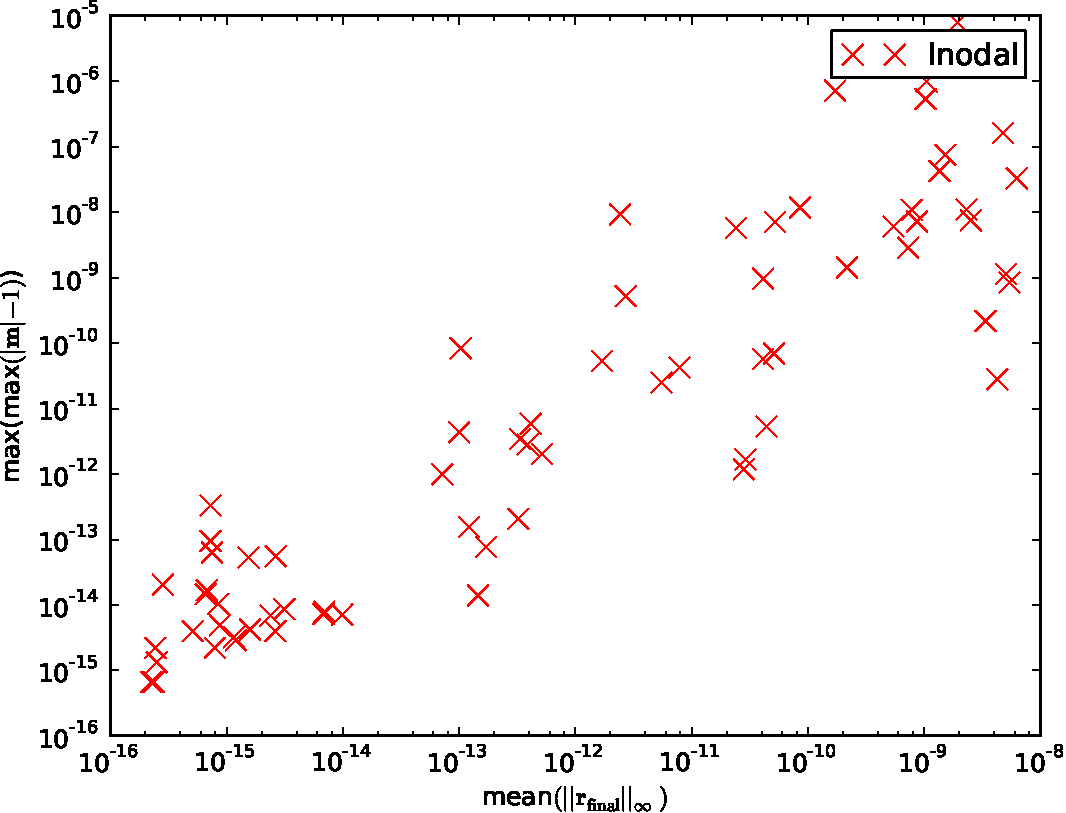
\includegraphics[width=0.8\textwidth]
  {plots/2d_wave_solution_m_length_newton_res/-maxmaxmathbfm-1vsmeanmathbfr_mathrmfinal_infty.pdf}
  \caption{Corrolation between maximum error of nodal magnetisation lengths and largest maximum Newton residual norm after convergence in the 2D wave example solved using adaptive IMR and nodal quadrature.}
  \label{fig:ml-error-2d-nodal-newton-tests}
\end{figure}


\begin{figure}
  \centering
  
\includegraphics[width=0.8\textwidth] {images/placeholder}
  \caption{Corrolation between error in energy and largest maximum Newton residual after convergence in the undamped 2D wave example solved using adaptive IMR and nodal quadrature.}
  \label{fig:energy-error-2d-nodal-newton-tests}
\end{figure}



\subsection{Conclusions}

We have shown that the conservation properties of IMR persist in a weak form FEM model when used with a nodal quadrature scheme and certain meshes.
??ds triangle mesh?



\section{The \mumag standard problem 4}

Widely used to test micromagnetic codes

Reversal of a thin film of permalloy under two different fields

Unfortunately FEM/BEM magnetostatic calcultations are extremely unsuited to thin film problems (the dense BEM matrix size is proportional to the size of the boundary, in thin films the entire problem is on the boundary. The additional geometric flexibility is not needed for simple cubeoid shapes.)
But we will do it anyway in order to test our results.

??ds mention that LL form of LLG is used for explicit step in IMR, mention CG + ... solver, diagonal mass matrix with nodal integration, .... Or move elsewhere?


\subsection{Problem specification}

The problem specification is as follows:

The magnetic domain is a simple sheet of magnetic material $500 \times 125 \times 3$nm with material parameters
\begin{equation}
  \begin{aligned}
    A &= 1.3\E{-11} \text{J/m}, \\
    M_s &= 8.0\E{5} \text{A/m}, \\
    \Kone &= 0.0, \\
    \gymagc &= 2.211 \E{5} \text{m/As}, \\
    \dampc &= 0.02.
  \end{aligned}
\end{equation}
Two different applied fields should be used, correspond to two different solutions:
\begin{equation}
  \begin{aligned}
    \happ_1 = [-24.6, 4.3, 0.0] \E{-3}\text{A/m}, \\
    \happ_1 = [-35.5, -6.3, 0.0] \E{-3}\text{A/m}, \\
  \end{aligned}
  \label{eq:mumag-h-app}
\end{equation}
where we have converted from the magnetic flux intensity specified by the \mumag website to magnetic field by dropping a factor of $\mu_0$ from the RHS.
The initial condition is the result of relaxing the magnetisation from the state created by a saturating field in the $[1,1,1]$.

The magnetic parameters result in a magnetostatic exchange length (and simulation unit length) of
\begin{equation}
  l_{\text{ex}} = \sqrt{\frac{2A}{\mu_0 M_s^2}} = 5.6858\text{nm},
\end{equation}
hence the normalised dimensions are $500 \times 125 \times 3 / 5.6858$.
The unit time is
\begin{equation}
  t_{\text{unit}} = \frac{1}{\gymagc M_s} = 5.653\text{ps}.
\end{equation}
The normalised applied fields are simply the fields given in \cref{eq:mumag-h-app} divided by $M_s = 8.0\E{5}$.

\subsection{Numerical methods and parameters}

Mesh

Newton tol

quadrature(s)

time integrator(s)

solvers

etc.


\subsection{Results}

Plot dynamics with some other peoples.

Conservation properties of IMR.


\subsection{Conclusions}

Semi-implicit causes problems with TR stability, IMR energy conservation.


\section{Reversal of a magnetic nanotube?}

More relevant problem for FEM/BEM methods--non-trivial geometry.

More relevant for conservation properties: complex, long time dynamics.


\subsection{Problem specification}

??ds


\subsection{Numerical methods and parameters}

??ds mesh generation



\subsection{Results}

??ds convergence: space and time


??ds conservation: m and energy


??ds adaptivity


??ds comparison to other methods?


%%% Local Variables:
%%% mode: latex
%%% TeX-master: "main"
%%% End:
